\newif\ifvimbug
\vimbugfalse

\ifvimbug
\begin{document}
\fi

\exercise{Non-parametric Density Estimation}
 
In this exercise, you will use the datasets \texttt{nonParamTrain.txt} for training and \texttt{nonParamTest.txt} for evaluating the performance of your model.

\begin{questions}

%----------------------------------------------

\begin{question}{Histogram}{4}
Compute and plot the histograms using $0.02$, $0.5$, $2.0$ size bins.  
Intuitively, indicate which bin size performs the best in and explain why. Knowing only these three trials, would you be sure that the one you picked is truly the best one? Attach the plot of the histograms and a snippet of your code.


\begin{answer}
Intuitively, the bins of size 0.5 perform the best. They show sufficient details of the distribution without having gaps. However, it is theoretically possible that the underlying distribution looks like the one that results from the histogram of bin size 0.02.

%\begin{figure}
\centering 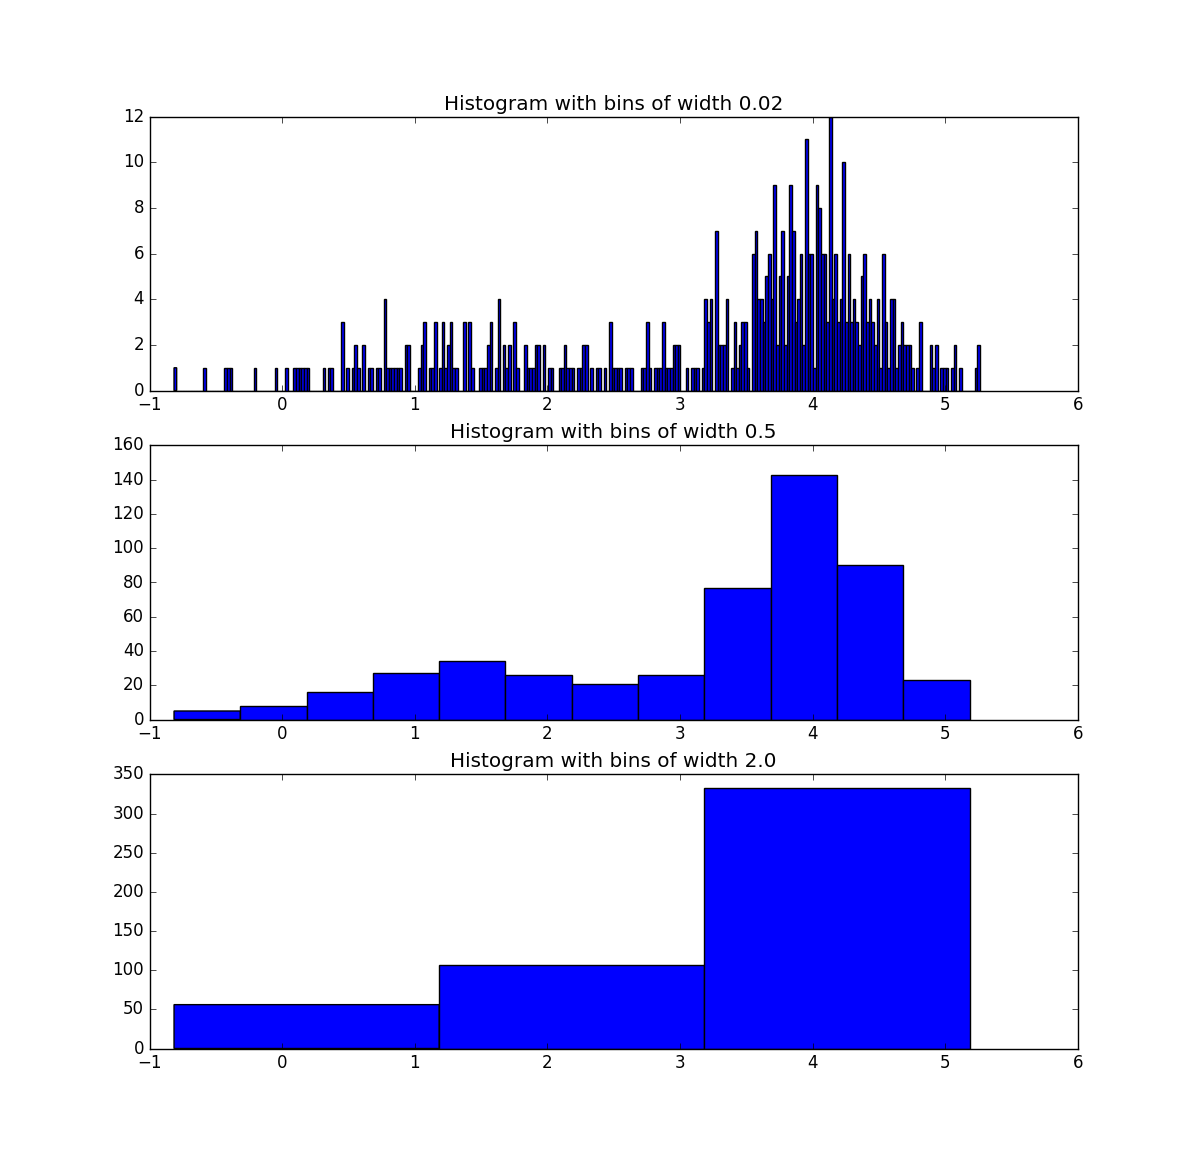
\includegraphics[width=0.6\linewidth]{dataSets/2-3-a}\label{fig:hist}
%\caption{Histrograms with various bin sizes}
%\label{fig:2-3-a}
%\end{figure}

\lstinputlisting[language=Python, firstline = 4]{dataSets/PythonProject/23a.py}


\end{answer}

\end{question}

%----------------------------------------------

\begin{question}{Kernel Density Estimate}{6}
Compute the probability density estimate using a Gaussian kernel with $\sigma=0.03$, $\sigma=0.2$ and $\sigma=0.8$. Compute the log-likelihood of the data for each case, compare them and show which parameter performs the best.
Generate a single plot with the different density estimates and attach it to your solutions. Plot the densities in the interval $x \in [-4,8]$, attach a snippet of your code and comment the results.

\begin{answer}
	The plot shows that the distribution resulting from the lowest sigma 0.02 has the highest log-likelihood. The function first creates two large arrays that are subtracted from each other to calculate all values of the sum simultaneously and then performs further steps to calculate the probability values, according to the gaussian kernel. In order to calculate the log-likelihood, the distribution can be evaluated at the samples by setting evalat==sample. The logarithm of every element of the resulting vector has to be taken and then summed up.
	
	\centering 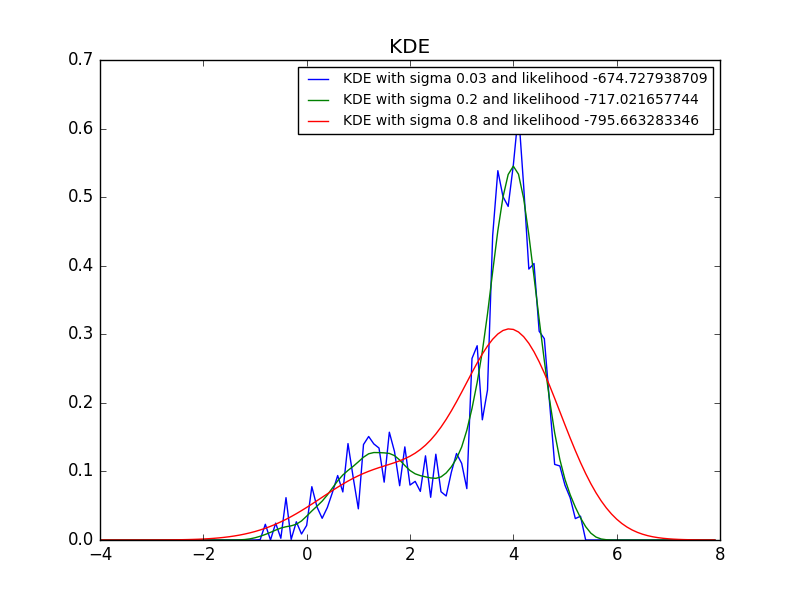
\includegraphics[width=0.6\linewidth]{dataSets/2-3-b}\label{fig:kde}

	
	\lstinputlisting[language=Python, firstline = 5, lastline = 21]{dataSets/PythonProject/23b.py}
\end{answer}

\end{question}

%----------------------------------------------

\begin{question}{K-Nearest Neighbors}{6}
Estimate the probability density with the K-nearest neighbors method with $K=2, K=8, K=35$.
Generate a single plot with the different density estimates and attach it to your solutions. Plot the densities in the interval $x \in [-4,8]$, attach a snippet of your code and comment the results.
(Note: you need to normalize your solution according to $K$ as the volume is not constant.)


\begin{answer}
	
		\centering 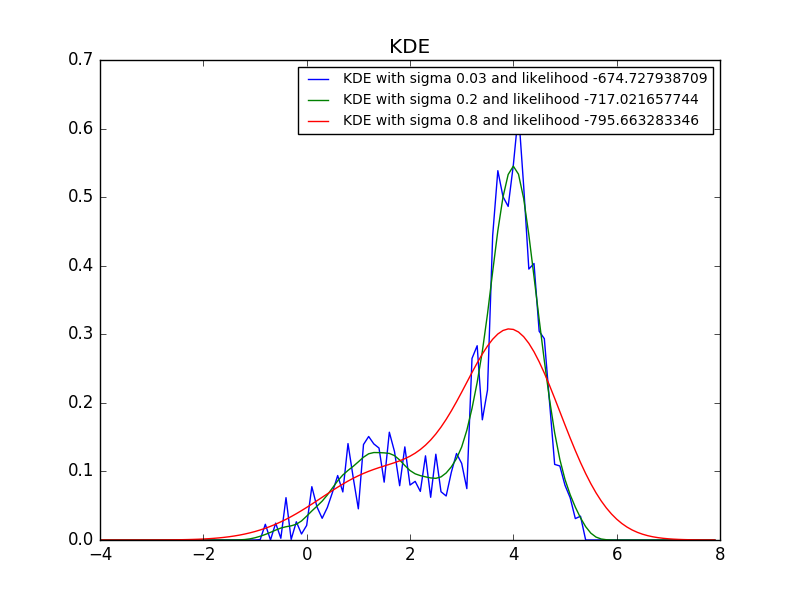
\includegraphics[width=0.6\linewidth]{dataSets/2-3-b}\label{fig:kde}
		
		
		\lstinputlisting[language=Python, firstline = 5, lastline = 21]{dataSets/PythonProject/23c.py}
\end{answer}

\end{question}

%----------------------------------------------

\begin{question}{Comparison of the Non-Parametric Methods}{4}
Estimate the log-likelihood of the testing data using the KDE estimators and the K-NN estimators.
Why do we need to test them on a different data set? Compare the log-likelihoods of the estimators w.r.t. both the training and testing sets in a table. Which estimator would you choose?

\begin{answer}
\end{answer}

\end{question}

\end{questions}
